%%%%%%%%%%%%%%%%%%%%%%%%%%%%%%%%%%%%%%%%%%%%%%%%%%%%%%%%%%%%%%
%% Modèle de présentation Beamer, doublé d'un court exemple/tutoriel.
%% Vincent Labatut 2017-19 <vincent.labatut@univ-avignon.fr>
%%%%%%%%%%%%%%%%%%%%%%%%%%%%%%%%%%%%%%%%%%%%%%%%%%%%%%%%%%%%%%
% réglages de beamer
\documentclass[10pt,    % taille de la police (défaut : 11pt)
%    handout,           % désactive les animations, et met la console en inverse vidéo
    french,             % langue de la présentation (thème prévu uniquement pour french & english)
    xcolor=table,       % couleur dans les tableaux
    envcountsect        % numéro de section dans les numéros des théorèmes
]{beamer}

%%%%%%%%%%%%%%%%%%%%%%%%%%%%%%%%%%%%%%%%%%%%%%%%%%%%%%%%%%%%%%
% réglages du thème
%\usepackage{au/sty/beamerthemeAU}          % pas d'option
\usepackage[light]{au/sty/beamerthemeAU}    % l'option "light" change les pages de titre et de section

%%%%%%%%%%%%%%%%%%%%%%%%%%%%%%%%%%%%%%%%%%%%%%%%%%%%%%%%%%%%%%
% réglages des notes
\usepackage{pgfpages}               % commenter les 3 lignes ci-dessous pour cacher les commentaires
%\setbeameroption{show notes}       % affiche les commentaires dans des slides intercalés
%\setbeameroption{show only notes}  % n'affiche que les slides de commentaires
%\setbeameroption{show notes on second screen=right} % (ou right, left, top, bottom) affiche les notes sur le côté, pour projection en double-écran

%%%%%%%%%%%%%%%%%%%%%%%%%%%%%%%%%%%%%%%%%%%%%%%%%%%%%%%%%%%%%%
% nom du fichier biblatex contenant la bibliographie
\addbibresource{biblio.bib}







%%%%%%%%%%%%%%%%%%%%%%%%%%%%%%%%%%%%%%%%%%%%%%%%%%%%%%%%%%%%%%
% titre et sous-titre de la présentation (le dernier est optionnel)
\title[Titre court] % à laisser vide si on ne veut rien afficher dans le pied-de-page
    {Exemple de titre de présentation particulièrement long, à tel point qu'il occupe plusieurs lignes sur la page de titre}
\subtitle{Il est également possible de définir un sous-titre relativement long, comme celui-ci}
%%%%%%%%%%%%%%%%%%%%%%%%%%%%%%%%%%%%%%%%%%%%%%%%%%%%%%%%%%%%%%
% date de la présentation
\date[Date courte]  % à laisser vide si on ne veut rien afficher dans le pied-de-page
    {\today}        % à laisser vide si on ne veut pas de date du tout, le défaut étant la date courante
%%%%%%%%%%%%%%%%%%%%%%%%%%%%%%%%%%%%%%%%%%%%%%%%%%%%%%%%%%%%%%
% auteurs et affiliations (ces dernières sont optionnelles)
\author[Auteur court] % à laisser vide si on ne veut rien afficher dans le pied-de-page
{PrénomA~NomA\inst{1} \and \underline{PrénomB~NomB}\inst{2} \and PrénomC~NomC\textsuperscript{1,2}}
\institute[] % (la version courte des affiliations n'est pas utilisée dans ce thème)
{\inst{1} Laboratoire Informatique d'Avignon -- LIA EA 4128 \texttt{\{prénom.nom\}@univ-avignon.fr}
\and \inst{2} Institut d'Innovation Disruptive, Université de l'Excellence \texttt{\{prénom.nom\}@univ-excell.fr}
}
%%%%%%%%%%%%%%%%%%%%%%%%%%%%%%%%%%%%%%%%%%%%%%%%%%%%%%%%%%%%%%
% optionnel : logo additionnel, par exemple labo
\titlegraphic{
\includegraphics[width=3cm,]{images/lia_logo.pdf}}
% pour insérer plusieurs logos, il faut les mettre dans une boîte comme ci-dessous
%\titlegraphic{\parbox{3cm}{
\includegraphics[width=3cm,]{images/ceri_logo.pdf}\newline
\includegraphics[width=3cm,]{images/lia_logo.pdf}}}
%%%%%%%%%%%%%%%%%%%%%%%%%%%%%%%%%%%%%%%%%%%%%%%%%%%%%%%%%%%%%%









%%%%%%%%%%%%%%%%%%%%%%%%%%%%%%%%%%%%%%%%%%%%%%%%%%%%%%%%%%%%%%
\begin{document}
%%% title page
\begin{frame}
  \titlepage
\end{frame}

%%% page d'introduction
\begin{frame}
    \label{frm:first}
    \frametitle{Présentation} 
    
    Ceci est une adaptation non-officielle du modèle officiel d'\href{http://univ-avignon.fr/}{Avignon Université}, initialement proposé uniquement aux formats \href{https://en.wikipedia.org/wiki/Microsoft\_PowerPoint}{MS PowerPoint} et \href{https://en.wikipedia.org/wiki/LibreOffice\#Included\_applications}{LO Impress}, à l'adresse  suivante (accès réservé):
    
    \url{https://e-doc.univ-avignon.fr/maison-de-la-communication/charte-graphique-de-luniversite/}
    
    \vspace{0.25cm}
    De plus, cette présentation montre comment utiliser les fonctionnalités basiques de \href{https://en.wikipedia.org/wiki/Beamer_(LaTeX)}{Beamer}, en supposant que le lecteur maîtrise déjà \LaTeX{}. Un tutoriel plus complet (et general) sur \LaTeX{} est disponible ici: 
    
    \url{https://www.overleaf.com/latex/templates/modele-rapport-uapv/pdbgdpzsgwrt}

    \vspace{0.25cm}
    La version anglaise de ces diapositives s'obtient en compilant \texttt{main\_EN.tex} au lieu de \texttt{main\_FR.tex}.
\end{frame}

%%% table des matières générée automatiquement
\begin{frame}{Plan de la présentation}
    \tableofcontents
%        [hideallsubsections] % ligne à dé-commenter pour cacher les sous-section dans la table des matières
\end{frame}












%%%%%%%%%%%%%%%%%%%%%%%%%%%%%%%%%%%%%%%%%%%%%%%%%%%%%%%%%%%%%%
\section{Fonctionnalités basiques}
\label{sec:basics}
\sectionframe

%%%%%%%%%%%%%%%%%%%%%%%%%%%%%%
\subsection{Classe, pages \& sections}
%%%
\begin{frame}
    \frametitle{Classe Beamer \& thème AU}
    
    La classe Beamer originale accepte un certain nombre d'options, notamment :
    \begin{itemize}
        \item \texttt{handout} : désactive les animations (cf. Section~\ref{sec:animations}) ;
        \item Taille du texte normal : le défaut est \texttt{11pt}.
    \end{itemize}

    \vspace{0.25cm}
    Le thème Beamer AU qui est proposé ici, \texttt{beamerthemeAU}, accepte en plus une option \texttt{light}, qui change l'aspect de la page de titre et des pages de section.
\end{frame}

%%%
\begin{frame}
    \frametitle{Pages : il est possible de définir de longs titres s'étendant sur deux lignes, comme ici} 
    
    Dans Beamer, une page de la présentation est appelée un \textit{frame}, et peut être définie grâce à l'environnement \texttt{frame}.
    
    \vspace{0.25cm}
    Le titre et le sous-titre d'une page sont respectivement définis via les commandes \texttt{\textbackslash{}title} et \texttt{\textbackslash{}subtitle}. Le sous-titre peut être omis, comme dans cette page. Cf. la page suivante pour voir un exemple de sous-titre.
    
    \vspace{0.25cm}
    L'environnement \texttt{frame} accepte un certain nombre d'options, parmi lesquelles: 
    \begin{itemize}
        \item \texttt{plain} : page nue, i.e. sans fond, en-tête, ni bas-de-page ;
        \item \texttt{allowframebreaks} : découpe automatiquement un contenu trop long en plusieurs pages (ex. bibliographie, Section~\ref{sec:biblio});
%        \item \texttt{shrink}: texte plus compact, pour les frames verbeux ; % ce thème n'offre pas cette option
        \item \texttt{fragile} : pour utiliser des environnements de type \textit{verbatim} (ex. \texttt{listings}, Page~\ref{frm:sourcecode});
        \item Alignement vertical : \texttt{c} (centré), \texttt{t} (haut) or \texttt{b} (bas).
    \end{itemize}
\end{frame}

%%%
\begin{frame}
    \frametitle{Sections} 
    \framesubtitle{Il est possible d'insérer un sous-titre sous le titre de la page, et celui-ci peut aussi s'étendre sur deux lignes si besoin}
    
    Les sections et sous-sections sont traitées comme dans un document \LaTeX{} classique, i.e. respectivement avec les commandes \texttt{\textbackslash{}section} et \texttt{\textbackslash{}subsection}.
    
    \vspace{0.25cm}
    Grâce à la commande \texttt{\textbackslash{}tableofcontents}, on peut automatiquement remplir une page avec la table des matières. L'option \texttt{hideallsubsections} permet d'exclure les sous-sections.
    
    \vspace{0.25cm}
    La commande \texttt{\textbackslash{}sectionframe} peut être utilisée pour insérer une page contenant seulement le titre de la section courante, ex. Section~\ref{sec:basics}.
\end{frame}




%%%%%%%%%%%%%%%%%%%%%%%%%%%%%%
\subsection{Mise en forme}
%%%
\begin{frame}
    \frametitle{Mise en forme du texte}
    
    Comme dans les documents \LaTeX{} classiques, on peut mettre le texte en \textit{italique} (\texttt{\textbackslash{}textit}) ou en \textbf{gras} (\texttt{\textbackslash{}textbf}), et même les \textit{\textbf{deux à la fois}} (en combinant ces deux commandes). On peut encore utiliser une police de caractères \texttt{à chasse fixe} (\texttt{\textbackslash{}texttt}).
    
    \vspace{0.25cm}
    Il est également possible d'utiliser la commande \texttt{\textbackslash{}alert}, qui est spécifique à Beamer, afin d'ajouter de la couleur, comme ici : \alert{Alerte !}
    
    \vspace{0.25cm}
    Le point médian utilisé pour l'écriture inclusive s'obtient avec la commande \texttt{\textbackslash{}textperiodcentered}, ou \texttt{\textbackslash{}tpc} pour faire plus court. Par exemple : chercheur\textperiodcentered{}se\tpc{}s. L'utilisateur·rice peut aussi l'insérer directement, par exemple via un copier-coller.
\end{frame}
    
%%%
\begin{frame}
    \frametitle{Citations verbatim}
    
    \vspace{0.25cm}
    On peut citer du texte via l'environnement \texttt{verse}, par exemple :
    \begin{verse}
        Citation, n.f. : action de répéter de façon erronée les mots d’un autre. \\ 
        \vspace{-0.5cm}
        \begin{flushright}--A. Bierce\end{flushright}
    \end{verse}
    
    Ou bien l'environnement \texttt{quote}, par exemple :
    \begin{quote}
        Fais un feu pour un homme, il aura chaud une journée. Mets le feu à un homme, il aura chaud pour le restant de sa vie. \\ 
        \vspace{-0.5cm}
        \begin{flushright}--T. Pratchett\end{flushright}
    \end{quote}
\end{frame}
    
%%%
\begin{frame}
    \frametitle{Expressions mathématiques}
    
    Les équations \textit{en-ligne} sont définies avec \texttt{\$}, comme dans les documents \LaTeX{} classiques. Par exemple : \texttt{\$f(x) = ax + b\$} donne $f(x)=ax + b$.
    
    \vspace{0.25cm}
    Les équations \textit{hors-ligne}, qui sont numérotées, sont insérées en utilisant l'environnement \texttt{equation}, par exemple
    \begin{equation}
        \label{equ:affine}
        f(x) = ax + b.
    \end{equation}
\end{frame}




%%%%%%%%%%%%%%%%%%%%%%%%%%%%%%
\subsection{Colonnes, blocs \& listes}
%%%%
\begin{frame}
    \frametitle{Colonnes}
    
    \begin{columns}[T,totalwidth=\textwidth] % 
        \begin{column}{0.33\textwidth}
            Les environnements \texttt{columns} et \texttt{column} (cf. le code source de cette page), permettent de partager une page en plusieurs colonnes indépendantes. 
            
            Cela peut aider à définir la structure de la page.
        \end{column}
        
        \begin{column}{0.33\textwidth}
            Avec \texttt{columns}, les options \texttt{t}, \texttt{b}, \texttt{c}, \texttt{T} contrôlent l'alignement vertical, et \texttt{totalwidth} la largeur globale (cf. \href{https://tex.stackexchange.com/a/51509/31360}{cette page} pour plus de détails).
            
            La largeur de chaque colonne peut être spécifiée via le paramètre de \texttt{column}.
        \end{column}
        
        \begin{column}{0.33\textwidth}
            Il est possible d'insérer du texte, mais aussi des images, dans une colonne.
            \begin{figure}[H]
                \centering
                
\includegraphics[scale=1]{au/backgrounds/au_logo.pdf}
                \vspace{-0.5cm}
                \caption{Logo d'Avignon Université}
                \label{fig:AUlogo}
            \end{figure}
        \end{column}
    \end{columns}
\end{frame}

%%%%
\begin{frame}
    \frametitle{Blocs}
    \label{frm:blocks}
    
    Les blocs sont spécifiques à Beamer, et permettent de mettre certains points en exergue. Il y a trois types de blocs, de couleurs différentes :

    \begin{block}{Normal}
        Environnement \texttt{block} : les blocs utilisés par défaut.
    \end{block}

    \begin{alertblock}{Alerte}
        Environnement \texttt{alertblock} : pour les points particulièrement importants.
    \end{alertblock}

    \begin{exampleblock}{Exemple}
        Environnement \texttt{exampleblock}: pour illustrer un concept.
    \end{exampleblock}
\end{frame}

%%%%
\begin{frame}
    \frametitle{Listes}
    
    Les listes sont définies comme dans un document \LaTeX{} classique, grâce à la commande \texttt{\textbackslash{}item} et à l'un des trois environnements suivants :
    \begin{columns}[T,onlytextwidth]
        \begin{column}{0.33\textwidth}
            \texttt{itemize} :
            \begin{itemize}
                \item Pierre ;
                \begin{itemize}
                    \item Feuille ;
                    \begin{itemize}
                        \item Ciseaux.
                    \end{itemize}
                \end{itemize}
            \end{itemize}
        \end{column}
        \begin{column}{0.33\textwidth}
            \texttt{enumerate} :
            \begin{enumerate}
                \item Premier;
                \begin{enumerate}
                    \item Deuxième;
                    \begin{enumerate}
                        \item Troisième.
                    \end{enumerate}
                \end{enumerate}
            \end{enumerate}
        \end{column}
        \begin{column}{0.33\textwidth}
            \texttt{description} :
            \begin{description}
                \item[Yin] Yang.
                \item[Chaud] Froid.
            \end{description}
        \end{column}
    \end{columns}
    
    \vspace{0.25cm}
    À noter l'utilisation des environnements \texttt{columns} et \texttt{column} dans cette page.
\end{frame}



%%%%%%%%%%%%%%%%%%%%%%%%%%%%%%
\subsection{Commentaires supplémentaires}
%%%%
\begin{frame}
    \frametitle{Commentaires supplémentaires}
    \framesubtitle{Définition des commentaires}
    
    Il est possible d'associer des commentaires à chaque page, en utilisant la commande \texttt{\textbackslash{}note}, et en lui passant le texte en paramètre. On peut placer les commentaires :
    \note{Ceci est un commentaire. Il apparaît en premier dans le slide produit. }
    \begin{itemize}
        \item \textit{À l'intérieur} du frame : tous les commentaires présents dans le même frame sont concaténés dans le même slide de commentaire.
        \note[item]{Ce commentaire est inséré en tant qu'item d'une liste placée à la fin du slide de commentaire.}
        \item \textit{À l'extérieur} des frames : chaque commentaire constitue un slide de commentaire distinct.
    \end{itemize}
    \note{Ce commentaire apparaît en deuxième. }
    
    \vspace{0.25cm}
    \note[item]{Ce commentaire est le deuxième item de la liste.}
    La commande \texttt{\textbackslash{}note} possède deux options \texttt{item} (à l'intérieur d'un frame) et \texttt{itemize} (à l'extérieur), permettant toutes les deux d'organiser automatiquement les commentaires sous forme de liste insérée dans le slide de commentaire. Cf. les commentaires associés à ce frame pour plus de détails.
    \note[item]{Et ceci est le troisième item de la liste.}
    \note{Ceci est le commentaire final, qui sera placé \textit{avant} la liste. À noter que ces commentaires sont compatibles avec les animations, cf. Section~\ref{sec:animations}.}
\end{frame}

%%%%
\begin{frame}   
    \label{frm:dispnotes}
    \frametitle{Commentaires supplémentaires}
    \framesubtitle{Affichage des commentaires}
        
    \vspace{0.25cm}
    Plusieurs options de Beamer permettent de déterminer comment les commentaires sont affichés :
    \begin{itemize}
        \item \texttt{hide notes} (défaut) : ils sont masqués.
        \item \texttt{show notes}: ils apparaissent dans des pages additionnelles insérées entre les pages de présentation.
        \item \texttt{show only notes}: n'affiche que ces pages de commentaire.
        \item \texttt{show notes on second screen=right} (or \texttt{left}, \texttt{top}, \texttt{bottom}): élargit les pages grâce au package \href{https://ctan.org/pkg/pdfpages?lang=en}{\texttt{pgfpages}}, de manière à faire apparaître les commentaires sur un second écran. Pour bénéficier de cette fonctionnalité, il faut utiliser un logiciel de visualisation approprié pour projeter la présentation, comme \href{http://impressive.sourceforge.net/}{Impress!ve} ou \href{http://dspdfviewer.danny-edel.de/}{Dual-Screen PDF Viewer}.
    \end{itemize}
    
    \textbf{Remarque :} pour rendre visibles les commentaires associés à la page précédente, modifiez simplement l'option en début de document et recompilez. 
\end{frame}











%%%%%%%%%%%%%%%%%%%%%%%%%%%%%%%%%%%%%%%%%%%%%%%%%%%%%%%%%%%%%%
\section{Éléments flottants \& renvois}
\sectionframe

%%%%%%%%%%%%%%%%%%%%%%%%%%%%%%
\subsection{Figures \& tableaux}
%%%%
\begin{frame}
    \frametitle{Figures}
    
    On insère une figure avec l'environnement \texttt{figure}, comme dans un document \LaTeX{} classique.
    
    \begin{figure}[H]
        \centering
        
\includegraphics[scale=0.05]{images/lia_logo.pdf}
        \vspace{-0.5cm}
        \caption{Logo du Laboratoire Informatique d'Avignon}
        \label{fig:LIAlogo}
    \end{figure}
    
    \vspace{0.25cm}
    Pour une image stockée dans un \textit{fichier} (JPEG, BMP, PDF, PNG, etc.), comme ci-dessus, on utilise la commande \texttt{\textbackslash{}includegraphics}.
\end{frame}

%%%%
\begin{frame}
    \frametitle{Diagrammes}
    Outre des fichiers, les figures peuvent également contenir des \textit{diagrammes}, spécifiés grâce au package \href{https://ctan.org/pkg/pgf?lang=en}{\texttt{TikZ}} :

    \begin{figure}[H]
        \centering
        \resizebox{0.35\linewidth}{!}{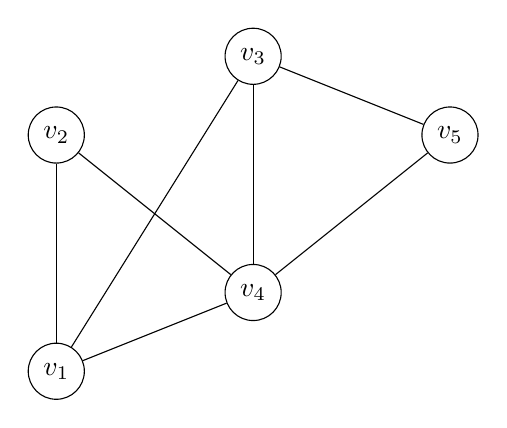
\begin{tikzpicture}
    % insert nodes
    \node[shape=circle,draw=black] (v1) at (0,0) {$v_1$};
    \node[shape=circle,draw=black] (v2) at (0,3) {$v_2$};
    \node[shape=circle,draw=black] (v3) at (2.5,4) {$v_3$};
    \node[shape=circle,draw=black] (v4) at (2.5,1) {$v_4$};
    \node[shape=circle,draw=black] (v5) at (5,3) {$v_5$} ;
    
    % insert links
	\draw (v1) -- (v2);
    \draw (v1) -- (v4);
	\draw (v1) -- (v3);
    \draw (v4) -- (v5);
    \draw (v3) -- (v4);
    \draw (v4) -- (v2);
    \draw (v5) -- (v3);
\end{tikzpicture}
}
        \hspace{0.25cm}\rulesep\hspace{0.25cm}
        \resizebox{0.45\linewidth}{!}{% Graphic for TeX using PGF
% Title: C:\Users\Vincent\Downloads\classdiag.dia
% Creator: Dia v0.97.2
% CreationDate: Mon Sep 24 11:08:38 2018
% For: Vincent
% \usepackage{tikz}
% The following commands are not supported in PSTricks at present
% We define them conditionally, so when they are implemented,
% this pgf file will use them.
\ifx\du\undefined
  \newlength{\du}
\fi
\setlength{\du}{15\unitlength}
\begin{tikzpicture}
\pgftransformxscale{1.000000}
\pgftransformyscale{-1.000000}
\definecolor{dialinecolor}{rgb}{0.000000, 0.000000, 0.000000}
\pgfsetstrokecolor{dialinecolor}
\definecolor{dialinecolor}{rgb}{1.000000, 1.000000, 1.000000}
\pgfsetfillcolor{dialinecolor}
\pgfsetlinewidth{0.100000\du}
\pgfsetdash{}{0pt}
\definecolor{dialinecolor}{rgb}{1.000000, 1.000000, 1.000000}
\pgfsetfillcolor{dialinecolor}
\fill (34.325000\du,11.850000\du)--(34.325000\du,13.250000\du)--(41.370000\du,13.250000\du)--(41.370000\du,11.850000\du)--cycle;
\definecolor{dialinecolor}{rgb}{0.000000, 0.000000, 0.000000}
\pgfsetstrokecolor{dialinecolor}
\draw (34.325000\du,11.850000\du)--(34.325000\du,13.250000\du)--(41.370000\du,13.250000\du)--(41.370000\du,11.850000\du)--cycle;
% setfont left to latex
\definecolor{dialinecolor}{rgb}{0.000000, 0.000000, 0.000000}
\pgfsetstrokecolor{dialinecolor}
\node at (37.847500\du,12.800000\du){Student};
\definecolor{dialinecolor}{rgb}{1.000000, 1.000000, 1.000000}
\pgfsetfillcolor{dialinecolor}
\fill (34.325000\du,13.250000\du)--(34.325000\du,16.650000\du)--(41.370000\du,16.650000\du)--(41.370000\du,13.250000\du)--cycle;
\definecolor{dialinecolor}{rgb}{0.000000, 0.000000, 0.000000}
\pgfsetstrokecolor{dialinecolor}
\draw (34.325000\du,13.250000\du)--(34.325000\du,16.650000\du)--(41.370000\du,16.650000\du)--(41.370000\du,13.250000\du)--cycle;
% setfont left to latex
\definecolor{dialinecolor}{rgb}{0.000000, 0.000000, 0.000000}
\pgfsetstrokecolor{dialinecolor}
\node[anchor=west] at (34.475000\du,13.950000\du){+name};
% setfont left to latex
\definecolor{dialinecolor}{rgb}{0.000000, 0.000000, 0.000000}
\pgfsetstrokecolor{dialinecolor}
\node[anchor=west] at (34.475000\du,14.750000\du){+firstname};
% setfont left to latex
\definecolor{dialinecolor}{rgb}{0.000000, 0.000000, 0.000000}
\pgfsetstrokecolor{dialinecolor}
\node[anchor=west] at (34.475000\du,15.550000\du){+age};
% setfont left to latex
\definecolor{dialinecolor}{rgb}{0.000000, 0.000000, 0.000000}
\pgfsetstrokecolor{dialinecolor}
\node[anchor=west] at (34.475000\du,16.350000\du){+gender};
\definecolor{dialinecolor}{rgb}{1.000000, 1.000000, 1.000000}
\pgfsetfillcolor{dialinecolor}
\fill (34.325000\du,16.650000\du)--(34.325000\du,17.650000\du)--(41.370000\du,17.650000\du)--(41.370000\du,16.650000\du)--cycle;
\definecolor{dialinecolor}{rgb}{0.000000, 0.000000, 0.000000}
\pgfsetstrokecolor{dialinecolor}
\draw (34.325000\du,16.650000\du)--(34.325000\du,17.650000\du)--(41.370000\du,17.650000\du)--(41.370000\du,16.650000\du)--cycle;
% setfont left to latex
\definecolor{dialinecolor}{rgb}{0.000000, 0.000000, 0.000000}
\pgfsetstrokecolor{dialinecolor}
\node[anchor=west] at (34.475000\du,17.350000\du){+register(course)};
\pgfsetlinewidth{0.100000\du}
\pgfsetdash{}{0pt}
\definecolor{dialinecolor}{rgb}{1.000000, 1.000000, 1.000000}
\pgfsetfillcolor{dialinecolor}
\fill (47.275000\du,16.750000\du)--(47.275000\du,18.150000\du)--(53.165000\du,18.150000\du)--(53.165000\du,16.750000\du)--cycle;
\definecolor{dialinecolor}{rgb}{0.000000, 0.000000, 0.000000}
\pgfsetstrokecolor{dialinecolor}
\draw (47.275000\du,16.750000\du)--(47.275000\du,18.150000\du)--(53.165000\du,18.150000\du)--(53.165000\du,16.750000\du)--cycle;
% setfont left to latex
\definecolor{dialinecolor}{rgb}{0.000000, 0.000000, 0.000000}
\pgfsetstrokecolor{dialinecolor}
\node at (50.220000\du,17.700000\du){Course};
\definecolor{dialinecolor}{rgb}{1.000000, 1.000000, 1.000000}
\pgfsetfillcolor{dialinecolor}
\fill (47.275000\du,18.150000\du)--(47.275000\du,19.950000\du)--(53.165000\du,19.950000\du)--(53.165000\du,18.150000\du)--cycle;
\definecolor{dialinecolor}{rgb}{0.000000, 0.000000, 0.000000}
\pgfsetstrokecolor{dialinecolor}
\draw (47.275000\du,18.150000\du)--(47.275000\du,19.950000\du)--(53.165000\du,19.950000\du)--(53.165000\du,18.150000\du)--cycle;
% setfont left to latex
\definecolor{dialinecolor}{rgb}{0.000000, 0.000000, 0.000000}
\pgfsetstrokecolor{dialinecolor}
\node[anchor=west] at (47.425000\du,18.850000\du){+name};
% setfont left to latex
\definecolor{dialinecolor}{rgb}{0.000000, 0.000000, 0.000000}
\pgfsetstrokecolor{dialinecolor}
\node[anchor=west] at (47.425000\du,19.650000\du){+year};
\definecolor{dialinecolor}{rgb}{1.000000, 1.000000, 1.000000}
\pgfsetfillcolor{dialinecolor}
\fill (47.275000\du,19.950000\du)--(47.275000\du,22.550000\du)--(53.165000\du,22.550000\du)--(53.165000\du,19.950000\du)--cycle;
\definecolor{dialinecolor}{rgb}{0.000000, 0.000000, 0.000000}
\pgfsetstrokecolor{dialinecolor}
\draw (47.275000\du,19.950000\du)--(47.275000\du,22.550000\du)--(53.165000\du,22.550000\du)--(53.165000\du,19.950000\du)--cycle;
% setfont left to latex
\definecolor{dialinecolor}{rgb}{0.000000, 0.000000, 0.000000}
\pgfsetstrokecolor{dialinecolor}
\node[anchor=west] at (47.425000\du,20.650000\du){+getContent()};
% setfont left to latex
\definecolor{dialinecolor}{rgb}{0.000000, 0.000000, 0.000000}
\pgfsetstrokecolor{dialinecolor}
\node[anchor=west] at (47.425000\du,21.450000\du){+getStudents()};
% setfont left to latex
\definecolor{dialinecolor}{rgb}{0.000000, 0.000000, 0.000000}
\pgfsetstrokecolor{dialinecolor}
\node[anchor=west] at (47.425000\du,22.250000\du){+getTeachers()};
\pgfsetlinewidth{0.100000\du}
\pgfsetdash{}{0pt}
\definecolor{dialinecolor}{rgb}{1.000000, 1.000000, 1.000000}
\pgfsetfillcolor{dialinecolor}
\fill (59.900000\du,11.850000\du)--(59.900000\du,13.250000\du)--(64.635000\du,13.250000\du)--(64.635000\du,11.850000\du)--cycle;
\definecolor{dialinecolor}{rgb}{0.000000, 0.000000, 0.000000}
\pgfsetstrokecolor{dialinecolor}
\draw (59.900000\du,11.850000\du)--(59.900000\du,13.250000\du)--(64.635000\du,13.250000\du)--(64.635000\du,11.850000\du)--cycle;
% setfont left to latex
\definecolor{dialinecolor}{rgb}{0.000000, 0.000000, 0.000000}
\pgfsetstrokecolor{dialinecolor}
\node at (62.267500\du,12.800000\du){Teacher};
\definecolor{dialinecolor}{rgb}{1.000000, 1.000000, 1.000000}
\pgfsetfillcolor{dialinecolor}
\fill (59.900000\du,13.250000\du)--(59.900000\du,14.250000\du)--(64.635000\du,14.250000\du)--(64.635000\du,13.250000\du)--cycle;
\definecolor{dialinecolor}{rgb}{0.000000, 0.000000, 0.000000}
\pgfsetstrokecolor{dialinecolor}
\draw (59.900000\du,13.250000\du)--(59.900000\du,14.250000\du)--(64.635000\du,14.250000\du)--(64.635000\du,13.250000\du)--cycle;
% setfont left to latex
\definecolor{dialinecolor}{rgb}{0.000000, 0.000000, 0.000000}
\pgfsetstrokecolor{dialinecolor}
\node[anchor=west] at (60.050000\du,13.950000\du){+discipline};
\definecolor{dialinecolor}{rgb}{1.000000, 1.000000, 1.000000}
\pgfsetfillcolor{dialinecolor}
\fill (59.900000\du,14.250000\du)--(59.900000\du,14.650000\du)--(64.635000\du,14.650000\du)--(64.635000\du,14.250000\du)--cycle;
\definecolor{dialinecolor}{rgb}{0.000000, 0.000000, 0.000000}
\pgfsetstrokecolor{dialinecolor}
\draw (59.900000\du,14.250000\du)--(59.900000\du,14.650000\du)--(64.635000\du,14.650000\du)--(64.635000\du,14.250000\du)--cycle;
\pgfsetlinewidth{0.100000\du}
\pgfsetdash{}{0pt}
\definecolor{dialinecolor}{rgb}{1.000000, 1.000000, 1.000000}
\pgfsetfillcolor{dialinecolor}
\fill (47.845000\du,3.850000\du)--(47.845000\du,5.250000\du)--(52.195000\du,5.250000\du)--(52.195000\du,3.850000\du)--cycle;
\definecolor{dialinecolor}{rgb}{0.000000, 0.000000, 0.000000}
\pgfsetstrokecolor{dialinecolor}
\draw (47.845000\du,3.850000\du)--(47.845000\du,5.250000\du)--(52.195000\du,5.250000\du)--(52.195000\du,3.850000\du)--cycle;
% setfont left to latex
\definecolor{dialinecolor}{rgb}{0.000000, 0.000000, 0.000000}
\pgfsetstrokecolor{dialinecolor}
\node at (50.020000\du,4.800000\du){Person};
\definecolor{dialinecolor}{rgb}{1.000000, 1.000000, 1.000000}
\pgfsetfillcolor{dialinecolor}
\fill (47.845000\du,5.250000\du)--(47.845000\du,8.650000\du)--(52.195000\du,8.650000\du)--(52.195000\du,5.250000\du)--cycle;
\definecolor{dialinecolor}{rgb}{0.000000, 0.000000, 0.000000}
\pgfsetstrokecolor{dialinecolor}
\draw (47.845000\du,5.250000\du)--(47.845000\du,8.650000\du)--(52.195000\du,8.650000\du)--(52.195000\du,5.250000\du)--cycle;
% setfont left to latex
\definecolor{dialinecolor}{rgb}{0.000000, 0.000000, 0.000000}
\pgfsetstrokecolor{dialinecolor}
\node[anchor=west] at (47.995000\du,5.950000\du){+name};
% setfont left to latex
\definecolor{dialinecolor}{rgb}{0.000000, 0.000000, 0.000000}
\pgfsetstrokecolor{dialinecolor}
\node[anchor=west] at (47.995000\du,6.750000\du){+firstname};
% setfont left to latex
\definecolor{dialinecolor}{rgb}{0.000000, 0.000000, 0.000000}
\pgfsetstrokecolor{dialinecolor}
\node[anchor=west] at (47.995000\du,7.550000\du){+age};
% setfont left to latex
\definecolor{dialinecolor}{rgb}{0.000000, 0.000000, 0.000000}
\pgfsetstrokecolor{dialinecolor}
\node[anchor=west] at (47.995000\du,8.350000\du){+gender};
\definecolor{dialinecolor}{rgb}{1.000000, 1.000000, 1.000000}
\pgfsetfillcolor{dialinecolor}
\fill (47.845000\du,8.650000\du)--(47.845000\du,9.050000\du)--(52.195000\du,9.050000\du)--(52.195000\du,8.650000\du)--cycle;
\definecolor{dialinecolor}{rgb}{0.000000, 0.000000, 0.000000}
\pgfsetstrokecolor{dialinecolor}
\draw (47.845000\du,8.650000\du)--(47.845000\du,9.050000\du)--(52.195000\du,9.050000\du)--(52.195000\du,8.650000\du)--cycle;
\pgfsetlinewidth{0.100000\du}
\pgfsetdash{}{0pt}
\pgfsetmiterjoin
\pgfsetbuttcap
{
\definecolor{dialinecolor}{rgb}{0.000000, 0.000000, 0.000000}
\pgfsetfillcolor{dialinecolor}
% was here!!!
\definecolor{dialinecolor}{rgb}{0.000000, 0.000000, 0.000000}
\pgfsetstrokecolor{dialinecolor}
\draw (50.020000\du,9.050000\du)--(50.020000\du,10.850000\du)--(37.847500\du,10.850000\du)--(37.847500\du,11.850000\du);
}
\definecolor{dialinecolor}{rgb}{0.000000, 0.000000, 0.000000}
\pgfsetstrokecolor{dialinecolor}
\draw (50.020000\du,9.961803\du)--(50.020000\du,10.850000\du)--(37.847500\du,10.850000\du)--(37.847500\du,11.850000\du);
\pgfsetmiterjoin
\definecolor{dialinecolor}{rgb}{1.000000, 1.000000, 1.000000}
\pgfsetfillcolor{dialinecolor}
\fill (50.420000\du,9.961803\du)--(50.020000\du,9.161803\du)--(49.620000\du,9.961803\du)--cycle;
\pgfsetlinewidth{0.100000\du}
\pgfsetdash{}{0pt}
\pgfsetmiterjoin
\definecolor{dialinecolor}{rgb}{0.000000, 0.000000, 0.000000}
\pgfsetstrokecolor{dialinecolor}
\draw (50.420000\du,9.961803\du)--(50.020000\du,9.161803\du)--(49.620000\du,9.961803\du)--cycle;
% setfont left to latex
\pgfsetlinewidth{0.100000\du}
\pgfsetdash{}{0pt}
\pgfsetmiterjoin
\pgfsetbuttcap
{
\definecolor{dialinecolor}{rgb}{0.000000, 0.000000, 0.000000}
\pgfsetfillcolor{dialinecolor}
% was here!!!
\definecolor{dialinecolor}{rgb}{0.000000, 0.000000, 0.000000}
\pgfsetstrokecolor{dialinecolor}
\draw (50.020000\du,9.050000\du)--(50.020000\du,10.850000\du)--(62.267500\du,10.850000\du)--(62.267500\du,11.850000\du);
}
\definecolor{dialinecolor}{rgb}{0.000000, 0.000000, 0.000000}
\pgfsetstrokecolor{dialinecolor}
\draw (50.020000\du,9.961803\du)--(50.020000\du,10.850000\du)--(62.267500\du,10.850000\du)--(62.267500\du,11.850000\du);
\pgfsetmiterjoin
\definecolor{dialinecolor}{rgb}{1.000000, 1.000000, 1.000000}
\pgfsetfillcolor{dialinecolor}
\fill (50.420000\du,9.961803\du)--(50.020000\du,9.161803\du)--(49.620000\du,9.961803\du)--cycle;
\pgfsetlinewidth{0.100000\du}
\pgfsetdash{}{0pt}
\pgfsetmiterjoin
\definecolor{dialinecolor}{rgb}{0.000000, 0.000000, 0.000000}
\pgfsetstrokecolor{dialinecolor}
\draw (50.420000\du,9.961803\du)--(50.020000\du,9.161803\du)--(49.620000\du,9.961803\du)--cycle;
% setfont left to latex
\pgfsetlinewidth{0.100000\du}
\pgfsetdash{}{0pt}
\pgfsetmiterjoin
\pgfsetbuttcap
{
\definecolor{dialinecolor}{rgb}{0.000000, 0.000000, 0.000000}
\pgfsetfillcolor{dialinecolor}
% was here!!!
\definecolor{dialinecolor}{rgb}{0.000000, 0.000000, 0.000000}
\pgfsetstrokecolor{dialinecolor}
\draw (37.847500\du,17.650000\du)--(37.847500\du,20.450000\du)--(47.275000\du,20.450000\du);
}
% setfont left to latex
\definecolor{dialinecolor}{rgb}{0.000000, 0.000000, 0.000000}
\pgfsetstrokecolor{dialinecolor}
\node at (42.561250\du,20.000000\du){Registers to};
\definecolor{dialinecolor}{rgb}{0.000000, 0.000000, 0.000000}
\pgfsetfillcolor{dialinecolor}
\fill (44.971250\du,20.100000\du)--(44.971250\du,19.700000\du)--(45.371250\du,19.900000\du)--cycle;
\definecolor{dialinecolor}{rgb}{0.000000, 0.000000, 0.000000}
\pgfsetstrokecolor{dialinecolor}
\node[anchor=west] at (38.047500\du,18.250000\du){1..*};
\definecolor{dialinecolor}{rgb}{0.000000, 0.000000, 0.000000}
\pgfsetstrokecolor{dialinecolor}
\node[anchor=east] at (47.075000\du,20.000000\du){5..*};
\pgfsetlinewidth{0.100000\du}
\pgfsetdash{}{0pt}
\pgfsetmiterjoin
\pgfsetbuttcap
{
\definecolor{dialinecolor}{rgb}{0.000000, 0.000000, 0.000000}
\pgfsetfillcolor{dialinecolor}
% was here!!!
\definecolor{dialinecolor}{rgb}{0.000000, 0.000000, 0.000000}
\pgfsetstrokecolor{dialinecolor}
\draw (62.267500\du,14.650000\du)--(62.267500\du,20.450000\du)--(53.165000\du,20.450000\du);
}
% setfont left to latex
\definecolor{dialinecolor}{rgb}{0.000000, 0.000000, 0.000000}
\pgfsetstrokecolor{dialinecolor}
\node at (57.716250\du,20.000000\du){teaches};
\definecolor{dialinecolor}{rgb}{0.000000, 0.000000, 0.000000}
\pgfsetfillcolor{dialinecolor}
\fill (56.168750\du,20.100000\du)--(56.168750\du,19.700000\du)--(55.768750\du,19.900000\du)--cycle;
\definecolor{dialinecolor}{rgb}{0.000000, 0.000000, 0.000000}
\pgfsetstrokecolor{dialinecolor}
\node[anchor=west] at (62.467500\du,15.250000\du){0..*};
\definecolor{dialinecolor}{rgb}{0.000000, 0.000000, 0.000000}
\pgfsetstrokecolor{dialinecolor}
\node[anchor=west] at (53.365000\du,20.000000\du){1..3};
\end{tikzpicture}
}
        \caption{Exemples de \textit{graphe} (à gauche) et de \textit{diagramme de classes} (à droite).}
        \label{fig:diagrams}
    \end{figure}
    
    \vspace{-0.5cm}
    Le diagramme de gauche a été défini manuellement, tandis que celui de droite a été produit via \href{http://dia-installer.de}{Dia}, un logiciel libre WYSIWYG capable d'exporter des diagrammes sous forme de code source \texttt{TikZ}.
\end{frame}
    
%%%%
\begin{frame}
    \frametitle{Tableaux}

    À l'instar des figures, les tableaux peuvent être insérés comme dans les documents \LaTeX{} classiques, grâce à l'environnement \texttt{table}.

    \begin{table}[H]
        \centering
    	\rowcolors{1}{fgVeryLightRed}{}
        \begin{tabular}{l r}
            \hline
	        \rowcolor{fgLightRed} 
            \textbf{Ville} & \textbf{Population} \\
            \hline
            Avignon, FR & 92~130 \\
            Avignon, QC & 15~246 \\
            Avignonet-Lauragais, FR & 1~443 \\
            Avignon-lès-Saint-Claude, FR & 390 \\
            Avignonet, FR & 194 \\
            \hline
        \end{tabular}
        \caption{Populations d'une sélection de villes.}
        \label{tab:population}
    \end{table}
    
    \textbf{Remarque :} on peut alternativement utiliser directement l'environnement \texttt{tabular}, car les légendes ne sont pas vraiment nécessaires dans une présentation.
\end{frame}
    
%%%%
\begin{frame}
    \frametitle{Tableaux CSV}

    Au lieu de définir manuellement le contenu d'un tableau, on peut le lire automatiquement et dynamiquement dans un fichier au format CSV, grâce au package \href{https://ctan.org/pkg/csvsimple?lang=en}{\texttt{csvsimple}} :

    \begin{table}[H]
    	\centering
    	\rowcolors{1}{fgVeryLightRed}{}
    	\begin{tabular}{l l l l r}
    		\hline
    		\rowcolor{fgLightRed} 
    		\textbf{Prénom} & \textbf{Patronyme} & \textbf{Nom de famille} & \textbf{Sexe} & \textbf{Âge} \\
    		\hline
    		\csvreader[head to column names, late after line=\\]
    		    {data/karamazov.csv}{}
                {\firstname & \middlename & \lastname & \sex & \age}
    		\hline
    	\end{tabular}
    	\caption{Contenu récupéré dans le fichier CSV \texttt{data/karamazov.csv}.}
    	\label{tab:csv}
    \end{table}
\end{frame}



%%%%%%%%%%%%%%%%%%%%%%%%%%%%%%
\subsection{Algorithmes \& code source}
%%%%
\begin{frame}
    \frametitle{Algorithmes}
    
    Il est possible de représenter des algorithmes sous forme de pseudocode, grâce à l'environnement \texttt{algorithm2e}, lui-même basé sur le package \href{https://ctan.org/pkg/algorithm2e?lang=en}{\texttt{algorithm2e}} :
    
    \begin{algorithm2e}[H]
        \DontPrintSemicolon             % masque les points-virgules dans le document
	    \KwData{$\ell$: liste}          % entrées de l'algo
	    \KwResult{$m$: maximum}         % sorties de l'algo
	
	    \BlankLine                      % sauter une ligne
	    \tcp{Initialisation}            % commentaires
	    $m \leftarrow -\infty$\;        % instruction élémentaire : attention au \; à la fin
	
	    \BlankLine
	    \tcp{Main loop}
	    \For{$i \leftarrow 1$ to length$(\ell)$}{%
		    \If{$\ell[i] > m$}{%
           	    $m  \leftarrow \ell[i]$\; \label{lne:example}
		    }
	    }
        % il y a de nombreuses commandes, correspondant à différents types de blocs
        % cf. la documentation du package pour plsu de détails 
        % https://ctan.org/pkg/algorithm2e?lang=en

    	\caption{Calcul du maximum d'une liste.}
        \label{alg:max}
    \end{algorithm2e}
\end{frame}

%%%%
\begin{frame}[fragile]
    \frametitle{Code source}
    \label{frm:sourcecode}
    
    On peut insérer du code source formaté correctement, grâce à l'environnement \texttt{lstlisting} du package \href{https://ctan.org/pkg/listings?lang=en}{\texttt{listings}} :
    
    \begin{lstlisting}[language=Java,caption={Applet Java Hello World.},label={lst:hello}]
// Hello.java
import javax.swing.JApplet;
import java.awt.Graphics;

public class Hello extends JApplet
{  public void paintComponent(Graphics g) 
   {  g.drawString("Hello: world!", 65, 95);
   }    
}
    \end{lstlisting}
    
    \vspace{0.25cm}
    \textbf{Remarque :} les frames contenant cet environnement doivent être définis en utilisant l'option \texttt{fragile}.
\end{frame}

%%%%
\begin{frame}[fragile]
    \frametitle{Contenu textuel \& console}
    
    Ce thème inclut deux environnements supplémentaires basés sur le package \href{https://ctan.org/pkg/framed?lang=en}{\texttt{framed}}.
    
    \vspace{0.25cm}
    Le premier, \texttt{filetext}, vise à afficher le contenu de fichiers textuels :
    
    \begin{filetext}
Première ligne du fichier texte ; \\
deuxième ligne, avec de la couleur \textcolor{fgRed}{ici} et \colorbox{fgRed}{là} ; \\
et enfin une troisième ligne.
    \end{filetext}
    
    \vspace{0.25cm}
    Le second environnement, \texttt{consoletext}, permet d'insérer du texte affiché dans un terminal :
    
    \begin{consoletext}
invite/>macommande monparametre \& \\
macommande: command not found \\
invite/>$\blacksquare$
    \end{consoletext}
    
    \vspace{0.25cm}
    \textbf{Remarque :} comme pour le code source (Page~\ref{frm:sourcecode}), il est nécessaire de spécifier l'option \texttt{fragile} lors de la création d'un frame contenant l'un de ces environnements.
\end{frame}







%%%%%%%%%%%%%%%%%%%%%%%%%%%%%%
\subsection{Éléments mathématiques}
%%%%
\begin{frame}
    \frametitle{Éléments flottants mathématiques}
    \small
    
    Beamer contient plusieurs environnements prédéfinis pour traiter différents concepts mathématiques : \texttt{theorem}, \texttt{corollary}, \texttt{definition}, \texttt{fact}, \texttt{example}, et \texttt{proof}. Ceux-ci sont rendus sous la forme de blocs (cf. Page~\ref{frm:blocks}):
    
    \begin{theorem}[Jörg Neunhäuserer]
        Dans tout sous-ensemble de $M = \{1, 2, ... , 2m\}$ contenant au moins $m + 1$ éléments, il existe deux nombres $a$, $b$ tels que $a$ divise $b$ \cite{Neunhauserer2013}.
        \label{th:theorem}
    \end{theorem} 
    
    L'option \texttt{envcountsect} de la classe Beamer permet d'ajouter le numéro de section dans la numérotation des théorèmes (et autres objets similaires), comme ci-dessus.
    
    \begin{proof}
         Soient $\{a_1, . . . , a_{m+1}\} \in M$ et la décomposition $a_i = 2^{r_i} q_i$, où les $q_i$ sont des nombres impairs. Il y a seulement $m$ nombres impairs dans $M$, donc un $q_i$ apparaît dans la décomposition de deux nombres $a_i$ et $a_j$ différents. Alors $a_i$ divise $a_j$ si $a_i < a_j$.
        \label{th:proof}
    \end{proof} 
\end{frame}
    




%%%%%%%%%%%%%%%%%%%%%%%%%%%%%%
\subsection{Renvois}
%%%
\begin{frame}
    \frametitle{Renvois généraux} 
    
    Les renvois fonctionnent comme dans les documents \LaTeX{} classiques, avec les commandes \texttt{\textbackslash{}label} et \texttt{\textbackslash{}ref}. Par exemple : Figure~\ref{fig:LIAlogo}, Table~\ref{tab:population}, Éq.(\ref{equ:affine}), Théorème~\ref{th:theorem}, Page~\ref{frm:first}, Algorithme~\ref{alg:max}, Ligne~\ref{lne:example} (dans un algorithme), Listing~\ref{lst:hello}.
    
    \vspace{0.25cm}
    Les hyperliens sont aussi définis comme dans un document \LaTeX{} classique, grâce au package \href{https://ctan.org/pkg/hyperref?lang=en}{hyperref}, et notamment à ses commandes \texttt{\textbackslash{}href} et \texttt{\textbackslash{}url} (ex. Page~\ref{frm:first}).
    
    \vspace{0.25cm}
    Les notes de bas de pages sont insérées via la commande classique \texttt{\textbackslash{}footnote}, comme ici\footnote{Une note de bas de page.}.
\end{frame}

%%%
\begin{frame}
    \frametitle{Références bibliographiques}
    
    Ce thème Beamer est configuré pour utiliser \href{https://ctan.org/pkg/biblatex?lang=en}{\texttt{BibLaTeX}} et \href{http://biblatex-biber.sourceforge.net/}{Biber} (au lieu du classique \href{http://www.bibtex.org/}{BibTeX}), ce qui résout toutes sortes de problèmes liés aux signes diacritiques (e.g. présence d'accents, cédilles ou autres dans les noms d'auteurs et titres d'articles).
    
    \vspace{0.25cm}
    Le fichier BibTeX lui-même est défini de façon classique, cf. \texttt{biblio.bib} pour un exemple. On peut utiliser les catégories bibliographiques classiques :
    
    \begin{table}[H]
        \small
        \centering
    	\rowcolors{1}{fgVeryLightRed}{}
        \begin{tabular}{l l r}
            \hline
	        \rowcolor{fgLightRed} 
            \textbf{Nature de la référence} & \textbf{Type BibTeX} & \textbf{Exemples}\\
            \hline
            Article de journal & \texttt{@Article} & \cite{Fortunato2010, Cossu2016} \\
            Article de conférence & \texttt{@InProceedings} & \cite{Wei1989, Mauttone2008} \\
            Monographie & \texttt{@Book} & \cite{Wolsey1998, Masuda2016} \\
            Chapitre de monographie & \texttt{@InBook} & \cite{Mainzer2007a, Reichardt2009a} \\
            Livre édité & \texttt{@Collection} & \cite{Pastor-Satorras2003a, Brandes2005} \\
            Chapitre de livre & \texttt{@InCollection} & \cite{Danon2007, Labatut2012a} \\
            Rapport technique & \texttt{@TechReport} & \cite{Rosvall2009a, Paraskevopoulos2013} \\
            Thèses de doctorat & \texttt{@PhDThesis} & \cite{Wong1978, Gerbaud2010} \\
            \hline
        \end{tabular}
        \caption{Principales catégories d'entrées bibliographies.}
        \label{tab:bibtex}
    \end{table}
\end{frame}

%%%
\begin{frame}
    \frametitle{Citations bibliographiques} 
    
    BibLaTeX offre plusieurs méthodes pour citer une référence bibliographique :
    \begin{itemize}
        \item La commande classique \texttt{\textbackslash{}cite}, ou de façon équivalente (dans ce contexte spécifique) \texttt{\textbackslash{}parencite}, insère seulement le code bibliographique : \cite{Labatut2012a} ;
        \item La commande \texttt{\textbackslash{}textcite} mentionne en plus les noms des auteurs : \textcite{Labatut2012a} ;
        \item La command \texttt{\textbackslash{}citeauthor} ne cite que les noms des auteurs : \citeauthor{Labatut2012a} ;
        \item La commande \texttt{\textbackslash{}footfullcite} insère la référence complète sur place, sous forme de note de bas de page\footfullcite{Labatut2012a}.
    \end{itemize}
\end{frame}










%%%%%%%%%%%%%%%%%%%%%%%%%%%%%%%%%%%%%%%%%%%%%%%%%%%%%%%%%%%%%%
\section{Superpositions \& animations}
\label{sec:animations}
\sectionframe

%%%%%%%%%%%%%%%%%%%%%%%%%%%%%%
\subsection{Introduction aux superpositions}
%%%%
\begin{frame}
    \frametitle{Notion de superposition}
    
    Les superpositions (overlays) permettent de dévoiler progressivement les différentes parties d'une page, au lieu de tout montrer en même temps. Cette fonctionnalité est assez semblable (bien que plus limitée) aux animations proposées dans MS Powerpoint et LO Impress.
    
    \vspace{0.25cm}
    Beamer propose deux façons de dissimuler les éléments constituant une page : 
    \begin{itemize}
        \item Les éléments \textit{voilés} apparaissent en filigrane ;
        \item Les éléments \textit{invisibles} sont complètement cachés.
    \end{itemize}
    
    \vspace{0.25cm}
    Chaque étape définie pour dévoiler les éléments de la page occasionne la création d'un slide spécifique dans le fichier de présentation final. Autrement dit, en présence de superpositions, un frame est rendu sous la forme de plusieurs slides.
\end{frame}

%%%%
\begin{frame}
    \frametitle{Pauses}
    
    La manière la plus simple d'utiliser les superpositions est la commande \texttt{\textbackslash{}pause}, que l'on place là où l'on veut arrêter le dévoilement de la page. Le reste de son contenu est alors \textit{voilé}.
    
    \vspace{0.25cm}
    Par exemple, voici une pause : \texttt{\textbackslash{}pause} \pause. Et voici la fin du paragraphe. Pour être précis, ce texte supplémentaire est placé sur un \textit{slide différent}, mais appartient au \textit{même frame} : le numéro de page dans le pied-de-page n'a pas changé.
    
    \vspace{0.25cm}
    \visible<3>{Il faut remarquer que, quand le texte ci-dessus est voilé, il est apparaît tout de même, mais en filigrane. Ceci peut être pratique, par exemple, si le présentateur ne se souvient pas de ce qui vient après \texttt{\textbackslash{}pause}.}
\end{frame}

%%%%%%%%%%%%%%%%%%%%%%%%%%%%%%
\subsection{Spécifications de superpositions}
%%%%
\begin{frame}
    \frametitle{Spécifications absolues de superpositions}
    \framesubtitle{Description}
    
    Beamer surcharge certaines commandes et environnements \LaTeX{} standard, afin qu'ils supportent des paramètres supplémentaires appelés \textit{spécifications de superpositions}. Ceux-ci permettent d'assigner des numéros aux différents éléments constituant la page. Après compilation, chacun de ces éléments apparaît l'un après l'autre, dans l'ordre spécifié. Chaque numéro correspond à un slide spécifique généré pour représenter l'évolution de la page considérée.
    
    \vspace{0.25cm}
    Ces paramètres ont la particularité de devoir être entourés de crochets pointus, par exemple \texttt{<3>} signifie que l'élément concerné apparaît dans le troisième slide de la page considérée. \visible<2->{Pour que l'élément reste visible dans les slides suivants, il est nécessaire d'ajouter un tiret : \texttt{<3->}.} \visible<3->{Il est aussi possible de provoquer sa disparition dans un slide ultérieur, ex. \texttt{<3-5>}.} \visible<4->{Enfin, on peut combiner ces intervalles temporels avec des virgules, ex. \texttt{<3-5,7-10,15>}.}
\end{frame}

%%%%
\begin{frame}
    \frametitle{Spécifications absolues de superpositions}
    \framesubtitle{Exemples}
    
    La commande \texttt{\textbackslash{}item} accepte les spécifications de superpositions, par exemple :
    \begin{itemize}
       \item<1> \texttt{\textbackslash{}item<1>}
       \item<2-3> \texttt{\textbackslash{}item<2-3>}
       \item<3-> \texttt{\textbackslash{}item<3->}
       \item<2,4> \texttt{\textbackslash{}item<2,4>}
    \end{itemize}
    
    \vspace{0.25cm}
    \visible<5->{Notez que la position des items est fixe, et indépendante du fait que les autres items soient cachés ou pas.}
    
    \vspace{0.25cm}
    \visible<6->{Les spécifications de superpositions ne concernent pas forcément la visibilité des éléments : cela dépend de la commande considérée. Par exemple : \textbf<7>{e.g. \texttt{\textbackslash{}textbf<7>}} \textcolor<8>{fgRed}{ou \texttt{\textbackslash{}textcolor<8>}}.}
\end{frame}

%%%%
\begin{frame}
    \frametitle{Spécifications relatives de superpositions}
    \framesubtitle{Opérateurs de base}

    Au lieu de donner explicitement des numéros de slides dans les spécifications, il est possible de procéder \textit{incrémentalement} grâce à l'opérateur \texttt{+}. Ce symbole est remplacé par la valeur courante du compteur de slides, \textit{puis} ce compteur est incrémenté de $1$. Par exemple, soient $C$ et $C'$ les valeurs courante et mise à jour du compteur, et $S$ le slide dans lequel l'élément apparaîtra :
    {\small\begin{itemize}
        \item<+-> \texttt{\textbackslash{}item<+->}: \makebox[1.5cm][l]{$C=1$,} \makebox[2.5cm][l]{$S=1$,} \makebox[2.5cm][l]{$C'=1+1=2$.}
        \item<+-> \texttt{\textbackslash{}item<+->}: \makebox[1.5cm][l]{$C=2$,} \makebox[2.5cm][l]{$S=2$,} \makebox[2.5cm][l]{$C'=2+1=3$.}
        \item<+-> \texttt{\textbackslash{}item<+->}: \makebox[1.5cm][l]{$C=3$,} \makebox[2.5cm][l]{$S=3$,} \makebox[2.5cm][l]{$C'=3+1=4$.}
    \end{itemize}}
    
    \vspace{0.15cm}
    Quand on utilise \texttt{.} à la place de \texttt{+}, le symbole est remplacé par la valeur courante du compteur \textit{moins un}, et ce compteur n'est \textit{pas} mis à jour. %Concrètement, cela permet de faire apparaître plusieurs éléments simultanément :
    {\small\begin{itemize}
        \item<+-> \texttt{\textbackslash{}item<+->}: \makebox[1.5cm][l]{$C=4$,} \makebox[2.5cm][l]{$S=4$,} \makebox[2.5cm][l]{$C'=4+1=5$.}
        \item<.-> \texttt{\textbackslash{}item<.->}: \makebox[1.5cm][l]{$C=5$,} \makebox[2.5cm][l]{$S=5-1=4$,} \makebox[2.5cm][l]{$C'=5$.}
        \item<+-> \texttt{\textbackslash{}item<+->}: \makebox[1.5cm][l]{$C=5$,} \makebox[2.5cm][l]{$S=5$,} \makebox[2.5cm][l]{$C'=5+1=6$.}
        \item<.-> \texttt{\textbackslash{}item<.->}: \makebox[1.5cm][l]{$C=6$,} \makebox[2.5cm][l]{$S=6-1=5$,} \makebox[2.5cm][l]{$C'=6$.}
    \end{itemize}}
\end{frame}

%%%%
\begin{frame}
    \frametitle{Spécifications relatives de superpositions}
    \framesubtitle{Décalages}
    On peut en plus préciser un \textit{décalage} après \texttt{+} or \texttt{.}, entre parenthèses. Il est utilisé pour modifier le compteur de slides, et sa valeur peut être aussi bien positive que négative.
    
    \vspace{0.25cm}
    Voici quelques exemples :
    \small{\begin{itemize}
        \item<+-> \makebox[2.25cm][l]{\texttt{\textbackslash{}item<+->}:} \makebox[1.5cm][l]{$C=1$,} \makebox[2.75cm][l]{$S=1$,} \makebox[2.5cm][l]{$C'=1+1=2$.}
        \item<+(1)-> \makebox[2.25cm][l]{\texttt{\textbackslash{}item<+(1)->}:} \makebox[1.5cm][l]{$C=2$,} \makebox[2.75cm][l]{$S=2+1=3$,} \makebox[2.5cm][l]{$C'=2+1=3$.}
        \item<+-> \makebox[2.25cm][l]{\texttt{\textbackslash{}item<+->}:} \makebox[1.5cm][l]{$C=3$,} \makebox[2.75cm][l]{$S=3$,} \makebox[2.5cm][l]{$C'=3+1=4$.}
        \item<+(2)-> \makebox[2.25cm][l]{\texttt{\textbackslash{}item<+(2)->}:} \makebox[1.5cm][l]{$C=4$,} \makebox[2.75cm][l]{$S=4+2=6$,} \makebox[2.5cm][l]{$C'=4+1=5$.}
        \item<+-> \makebox[2.25cm][l]{\texttt{\textbackslash{}item<+->}:} \makebox[1.5cm][l]{$C=5$,} \makebox[2.75cm][l]{$S=5$,} \makebox[2.5cm][l]{$C'=5+1=6$.}
        \item<+(-1)-> \makebox[2.25cm][l]{\texttt{\textbackslash{}item<+(-1)->}:} \makebox[1.5cm][l]{$C=6$,} \makebox[2.75cm][l]{$S=6-1=5$,} \makebox[2.5cm][l]{$C'=6+1=7$.}
        \item<.(1)-> \makebox[2.25cm][l]{\texttt{\textbackslash{}item<.(1)->}:} \makebox[1.5cm][l]{$C=7$,} \makebox[2.75cm][l]{$S=7-1+1=7$,} \makebox[2.5cm][l]{$C'=7$.}
        \item<+-> \makebox[2.25cm][l]{\texttt{\textbackslash{}item<+->}:} \makebox[1.5cm][l]{$C=7$,} \makebox[2.75cm][l]{$S=7$,} \makebox[2.5cm][l]{$C'=7+1=8$.}
    \end{itemize}}
\end{frame}




%%%%%%%%%%%%%%%%%%%%%%%%%%%%%%
\subsection{Commandes de superposition}
%%%%
\begin{frame}
    \frametitle{Principales commandes de superposition}
    \framesubtitle{Description}

    Il y a aussi des commandes Beamer spécifiques pour définir des superpositions. Elles prennent la forme générale \texttt{\textbackslash{}xxxxx<y>\{zzzz\}}, où \texttt{xxxxx} est la commande, \texttt{y} une spécification de superposition, et \texttt{zzzz} le contenu concerné.
    
    \vspace{0.25cm}
    Les trois commandes principales, listées ci-dessous, visent à afficher le contenu concerné sur les slides spécifiées, et à le cacher sur les autres slides. Elles diffèrent de par la façon dont elles masquent ce contenu :
    \begin{itemize}
        \item \texttt{\textbackslash{}visible} : le contenu caché est complètement \textit{invisible}.
        \item \texttt{\textbackslash{}uncover} : le contenu caché est simplement \textit{voilé}.
        \item \texttt{\textbackslash{}only}: le contenu caché est purement \textit{supprimé} de la page. 
    \end{itemize}
\end{frame}
    
%%%%
\begin{frame}[t]
    \frametitle{Principales commandes de superposition}
    \framesubtitle{Exemples}

    Voici une illustration de l'utilisation des commandes principales :
    
    \only<2>{Ce texte apparaît sur le 2ème slide via \texttt{\textbackslash{}only}.} 
    
    \uncover<3>{Ce texte apparaît sur le 3ème slide via \texttt{\textbackslash{}uncover}. Il remplace le texte précédent, car celui-ci avait été inséré avec \texttt{\textbackslash{}only}).} 
    
    \only<4>{Ce texte apparaît sur le 4ème slide via \texttt{\textbackslash{}only}. Il est placé après l'espace correspondant au texte précédent, qui avait été inséré avec \texttt{\textbackslash{}uncover}.} 
    
    \only<5>{Ce texte apparaît sur le 5ème slide également via \texttt{\textbackslash{}only}, à la place du texte précédent.} 
    
    \visible<6>{Ce texte apparaît sur le 6ème slide via \texttt{\textbackslash{}visible}, à la place du texte précédent.} 
    
    \visible<7>{Enfin, ce texte apparaît sur le 7ème slide également via \texttt{\textbackslash{}visible}, et seulement après l'espace laissé pour le texte précédent.}
\end{frame}

%%%%
\begin{frame}
    \frametitle{Autres commandes de superposition}
    
    La commande \texttt{\textbackslash{}invisible} est simplement le contraire de \texttt{\textbackslash{}visible} : elle rend le contenu concerné complètement invisible sur les slides spécifiés, et l'affiche sur les autres slides.
    
    \vspace{0.25cm}
    La commande \texttt{\textbackslash{}onslide} est relativement générique : elle prend un paramètre additionnel optionnel appelé \textit{modificateur}, et pouvant être \texttt{+} ou \texttt{*}. Pour faire simple :
    \begin{itemize}
        \item<1-> \texttt{\textbackslash{}onslide} se comporte comme \texttt{\textbackslash{}uncover};
        \item<2-> \texttt{\textbackslash{}onslide+} se comporte comme \texttt{\textbackslash{}visible};
        \item<3-> \texttt{\textbackslash{}onslide*} se comporte comme \texttt{\textbackslash{}only}. 
    \end{itemize}
    
    \vspace{0.25cm}
    La commande \texttt{\textbackslash{}alt} permet d'afficher différents contenus dans les slides spécifiés vs. les autres slides. Par exemple, \texttt{\textbackslash{}alt<1>\{slide\}\{autres\}} donne : \alt<1>{slide}{autres}.
    
    \vspace{0.25cm}
    La commande \texttt{\textbackslash{}temporal} est similaire, mais distingue les slides situées avant/pendant/après les spécifications de superposition. Par exemple, \texttt{\textbackslash{}temporal<2>\{avt\}\{pdt\}\{apr\}} donne : \temporal<2>{avt}{pdt}{apr}.
\end{frame}




%%%%%%%%%%%%%%%%%%%%%%%%%%%%%%
\subsection{Superpositions diverses}
%%%%
\begin{frame}
    \frametitle{Région modifiable de taille fixe}
    
    Il est possible de définir une région de taille fixe dans la page, dont le contenu est modifiable par superposition. L'intérêt est que le reste de la page ne bouge pas lorsque ce contenu évolue.
    
    \vspace{0.25cm}
    L'environnement \texttt{\textbackslash{}overlayarea} permet de spécifier les largeur et hauteur de cette région, tandis que l'environnement \texttt{\textbackslash{}overprint} requiert seulement sa largeur : la hauteur est ajustée automatiquement au plus haut contenu.
    
    \vspace{0.25cm}
    \begin{columns}[T,totalwidth=\textwidth] % 
        \begin{column}{0.49\textwidth}
            Voici un exemple basé sur \texttt{overlayarea} :
            
            \begin{overlayarea}{\textwidth}{2cm}
                \uncover<2>{Texte du 2ème slide.}
                \uncover<3>{Texte plus long situé sur le 3ème slide.}
            \end{overlayarea}
            
            Texte situé hors de la région.
        \end{column}
        \begin{column}{0.49\textwidth}
            Voici un exemple basé sur \texttt{overprint} :
            
            \begin{overprint}[\textwidth]
                \uncover<2>{Texte du 2ème slide.}
                \uncover<3>{Texte plus long situé sur le 3ème slide.}
            \end{overprint}
            
            Texte situé hors de la région.
        \end{column}
    \end{columns}
\end{frame}


%%%%
\begin{frame}
    \frametitle{Superpositions \& tableaux}
    \small
    Il est possible d'utiliser les commandes principales de superposition pour contrôler la visibilité des éléments constituant une table. Par exemple :
    
    \begin{table}[H]
        \centering
    	\rowcolors{1}{fgVeryLightRed}{}
        \begin{tabular}{l l l l l l}
            \hline
	        \rowcolor{fgLightRed} 
            \textbf{Organes} & \textbf{Centaure} & \textbf{Chimère} & \textbf{Minotaure} & \textbf{Sphinx} & \textcolor<3->{fgRed}{\textbf{Tarasque}} \\
            \textbf{Bœuf} & $\times$ & $\times$ & \checkmark & $\times$ & \textcolor<3->{fgRed}{\checkmark} \\
            \textbf{Cheval} & \checkmark & $\times$ & $\times$ & $\times$ & \textcolor<3->{fgRed}{\checkmark} \\
            \textbf{Chèvre} & $\times$ & \checkmark & $\times$ & $\times$ & \textcolor<3->{fgRed}{$\times$} \\
            \textbf{Dragon} & $\times$ & \checkmark & $\times$ & $\times$ & \textcolor<3->{fgRed}{\checkmark} \\
            \uncover<2->{\textbf{Humain} & \checkmark & $\times$ & \checkmark & \checkmark & \textcolor<3->{fgRed}{\checkmark} \\}
            \textbf{Lion} & $\times$ & \checkmark & $\times$ & \checkmark & \textcolor<3->{fgRed}{\checkmark} \\
            \textbf{Ours} & $\times$ & $\times$ & $\times$ & $\times$ & \textcolor<3->{fgRed}{\checkmark} \\
            \textbf{Scorpion} & $\times$ & $\times$ & $\times$ & $\times$ & \textcolor<3->{fgRed}{\checkmark} \\
            \textbf{Serpent} & $\times$ & \checkmark & $\times$ & $\times$ & \textcolor<3->{fgRed}{$\times$} \\
            \textbf{Tortue} & $\times$ & $\times$ & $\times$ & $\times$ & \textcolor<3->{fgRed}{\checkmark} \\
            \hline
        \end{tabular}
        \caption{Composition de diverses créatures légendaires.}
        \label{tab:creatures}
    \end{table}
\end{frame}

%%%%
\begin{frame}
    \frametitle{Superpositions \& diagrammes}
    Ce thème permet d'utiliser les superpositions dans les diagrammes \texttt{TikZ}, de manière à progressivement dévoiler certaines parties du diagramme, ou modifier ce diagramme d'autres façons. Pour cela, on utilise le paramètre \texttt{visible on} dans les options de la commande \texttt{TikZ} concernée. Sa valeur doit être une spécification de superpositions. Voici un exemple :
    
    \begin{columns}[totalwidth=\textwidth]
        \begin{column}{0.49\textwidth}
            Dans la figure, le sommet $v_1$ est dessiné avec :

            \texttt{\textbackslash{}node[shape=circle, draw=red, \alert{visible on=<2->}] (v1) at (0,0) \{\$v\_1\$\};}
            
            \vspace{0.25cm}
            Et ses arêtes avec :
	        
	        \texttt{\textbackslash{}draw[\alert{visible on=<2->}, draw=red] (v1) -- (v2);}
        \end{column}
        \begin{column}{0.49\textwidth}
            \begin{figure}[H]
                \centering
                \resizebox{0.6\linewidth}{!}{\begin{tikzpicture}
    % insert nodes
    \node[shape=circle,draw=red,visible on=<2->,text=red] (v1) at (0,0) {$v_1$};
    \node[shape=circle,draw=black] (v2) at (0,3) {$v_2$};
    \node[shape=circle,draw=black] (v3) at (2.5,4) {$v_3$};
    \node[shape=circle,draw=black] (v4) at (2.5,1) {$v_4$};
    \node[shape=circle,draw=black] (v5) at (5,3) {$v_5$} ;
    
    % insert links
    \draw (v4) -- (v5);
    \draw (v3) -- (v4);
    \draw (v4) -- (v2);
    \draw (v5) -- (v3);
	\draw[visible on=<2->,draw=red] (v1) -- (v2);
    \draw[visible on=<2->,draw=red] (v1) -- (v4);
	\draw[visible on=<2->,draw=red] (v1) -- (v3);
\end{tikzpicture}
}
                \caption{Superpositions dans un diagramme \texttt{TikZ}.}
                \label{fig:overlays}
            \end{figure}
        \end{column}
    \end{columns}
\end{frame}











%%%%%%%%%%%%%%%%%%%%%%%%%%%%%%%%%%%%%%%%%%%%%%%%%%%%%%%%%%%%%%
\highlightframe{Questions ?}

%%%%%%%%%%%%%%%%%%%%%%%%%%%%%%%%%%%%%%%%%%%%%%%%%%%%%%%%%%%%%%
\appendix
\section{Annexe}
\sectionframe

%%%%
\begin{frame}{Informations complémentaires}
	Il est possible d'utiliser la commande \texttt{\textbackslash{}appendix} pour créer des pages supplémentaires, par exemple pour servir de support lorsqu'on répond aux questions du public. 
	
    \vspace{0.25cm}
	Grâce au package \href{https://ctan.org/pkg/appendixnumberbeamer?lang=en}{\texttt{appendixnumberbeamer}}, ces pages supplémentaires ne sont pas prises en compte dans le numéro de page affiché dans le pied-de-page.
	
    \vspace{0.25cm}
	Les pages contenant les références bibliographiques ne sont pas comptées non plus.
\end{frame}

%%%%%%%%%%%%%%%%%%%%%%%%%%%%%%%%%%%%%%%%%%%%%%%%%%%%%%%%%%%%%%
\section{Références bibliographiques}
\label{sec:biblio}
\sectionframe

%%%%
\begin{frame}[t,allowframebreaks]
    \frametitle{Références bibliographiques}
    
    \printbibliography
\end{frame}



%%%%%%%%%%%%%%%%%%%%%%%%%%%%%%%%%%%%%%%%%%%%%%%%%%%%%%%%%%%%%%
\end{document}
